\documentclass[a4paper,12pt]{article}
\usepackage[spanish]{babel}
\spanishdecimal{.}
\selectlanguage{spanish}
\usepackage[spanish,onelanguage,ruled]{algorithm2e}
\usepackage[utf8]{inputenc}
\usepackage{siunitx}
\usepackage{graphicx}
\usepackage{caption}
\usepackage{subcaption}
\usepackage[top=2cm, bottom=2cm, left=2cm, right=2cm]{geometry}
\usepackage{hyperref}
\usepackage{verbatim}
\usepackage{amssymb}
\usepackage{mathtools}
\usepackage{listings}
\usepackage{color}
\definecolor{backcolour}{rgb}{0.95,0.95,0.92}
\newcommand\ddfrac[2]{\frac{\displaystyle #1}{\displaystyle #2}}
\lstset{backgroundcolor=\color{backcolour}, basicstyle=\footnotesize}
\lstset{xleftmargin=1cm, xrightmargin=1cm, breaklines=true}

\title{Práctica 5 \\ Conexión de sensores de luz, temperatura y batería a la tarjeta Arduino}
\author{Laboratorio de Bio-Robótica}
\date{Construcción de Robots Móviles}
\begin{document}
\renewcommand{\tablename}{Tabla}
\maketitle
\section*{Objetivos}
\begin{itemize}
\item Construir dos sensores de luz empleando fotorresistores (LDR).
\item Construir un sensor de batería empleando un divisor de voltaje.
\item Utilizar el circuito TMP36 para sensar temperatura.
\item Implementar un nodo de ROS en la tarjeta Arduino Uno que publique los valores  de dichos sensores. 
\item Utilizar una interfaz gráfica de usuario (GUI) para desplegar los valores de los sensores. 
\end{itemize}

\section{Introducción}
Un robot inteligente puede definirse como una máquina capaz de extraer información de su ambiente y usar el conocimiento de su mundo para moverse de forma segura y significativa con un propósito específico. Por ello, un robot debe contar con los sensores adecuados que le permitan obtener la información necesaria, ya sea de su estado interno o externo, para llevar a cabo su tarea. 

Existen varias formas de clasificar los sensores. Una de ellas los separa en activos y pasivos. Los sensores activos son aquellos que necesitan emitir energía para realizar la medición, por ejemplo, un sensor láser (laser range-finder) requiere emitir luz para calcular la distancia a los obstáculos. Los sensores de distancia construidos en la práctica 4 son también un ejemplo de sensores activos. Sonares y cámaras RGB-D necesitan emitir sonido y luz, respectivamente, para realizar sus mediciones. Los sensores pasivos, por el contrario, no requieren emitir energía para medir. Micrófonos y cámaras RGB son ejemplos de este tipo de sensores. 

Otra forma de clasificar los sensores es en propioceptivos y exteroceptivos. Los propioceptivos miden cantidades físicas relacionadas con el estado interno del robot, mientras que los exteroceptivos miden el estado externo. Encoders y sensores de batería son ejemplos de sensores propioceptivos. Cámaras, micrófonos y sensores láser son ejemplos de sensores exteroceptivos. 

Los resistores dependientes de luz (LDR, del inglés \textit{light-dependent resistor}) o fotorresistores son componentes cuya resistencia disminuye con el aumento de intensidad de la luz que incide sobre ellos. Cuando incide una luz intensa sobre un LDR, su resistencia puede disminuir hasta el orden de decenas de ohms, mientras que en la oscuridad, su resistencia puede aumentar hasta el orden de megaohms. Si un LDR se coloca en serie con una resistencia fija, se puede formar un divisor de voltaje cuya salida es función de la intensidad de la luz. 

Para medir el nivel de batería del robot, bastaría con leer su voltaje mediante un convertidor analógico-digital, sin embargo, dado que el Arduino Uno sólo puede convertir voltajes entre 0V y 5V y la batería del robot es de 7.4V nominales (con un máximo de 8.4V), es necesario utilizar un divisor de voltaje que reduzca la señal de la batería a la mitad. 

El TMP36 es un sensor de temperatura de precisión y bajo voltaje cuya salida es proporcional a la temperatura en grados Celsius. Este sensor es muy fácil de usar puesto que no requiere calibración y el voltaje de salida puede ser convertido fácilmente a temperatura utilizando el factor de escala de 10 mV/\si{\degree}C.

En esta praćtica se construirán dos sensores de luz y uno de batería, todos ellos sensores pasivos. Los sensores de luz se clasifican como exteroceptivos y el de batería, como interoceptivo. También se utilizará el sensor de temperatura TMP36, que entra en la clasificación de pasivo y exteroceptivo. 

\section{Desarrollo}
\subsection{Sensores de luz}
Construya dos sensores de luz utilizando el circuito que se muestra en la figura \ref{fig:LDR}. En este circuito, la salida $V_o$ está dada por
\[V_o = \frac{R_1}{R_{LDR} + R_1}V_{cc}\]
donde $R_{LDR}$ es la resistencia del LDR, que cambia con respecto a la intensidad de la luz y $R_1$ es una resistencia de valor fijo. Como se observa en la figura \ref{fig:LDRVo}, la salida no es lineal con respecto a la entrada, por lo que si se desea obtener una medida de la intensidad de luz a partir del voltaje medido, es necesario realizar una corrección no lineal. Para las tareas que desempeñará el robot no es necesaria dicha corrección. 
\begin{figure}
  \centering
  \begin{subfigure}[b]{0.43\textwidth}
    \centering
    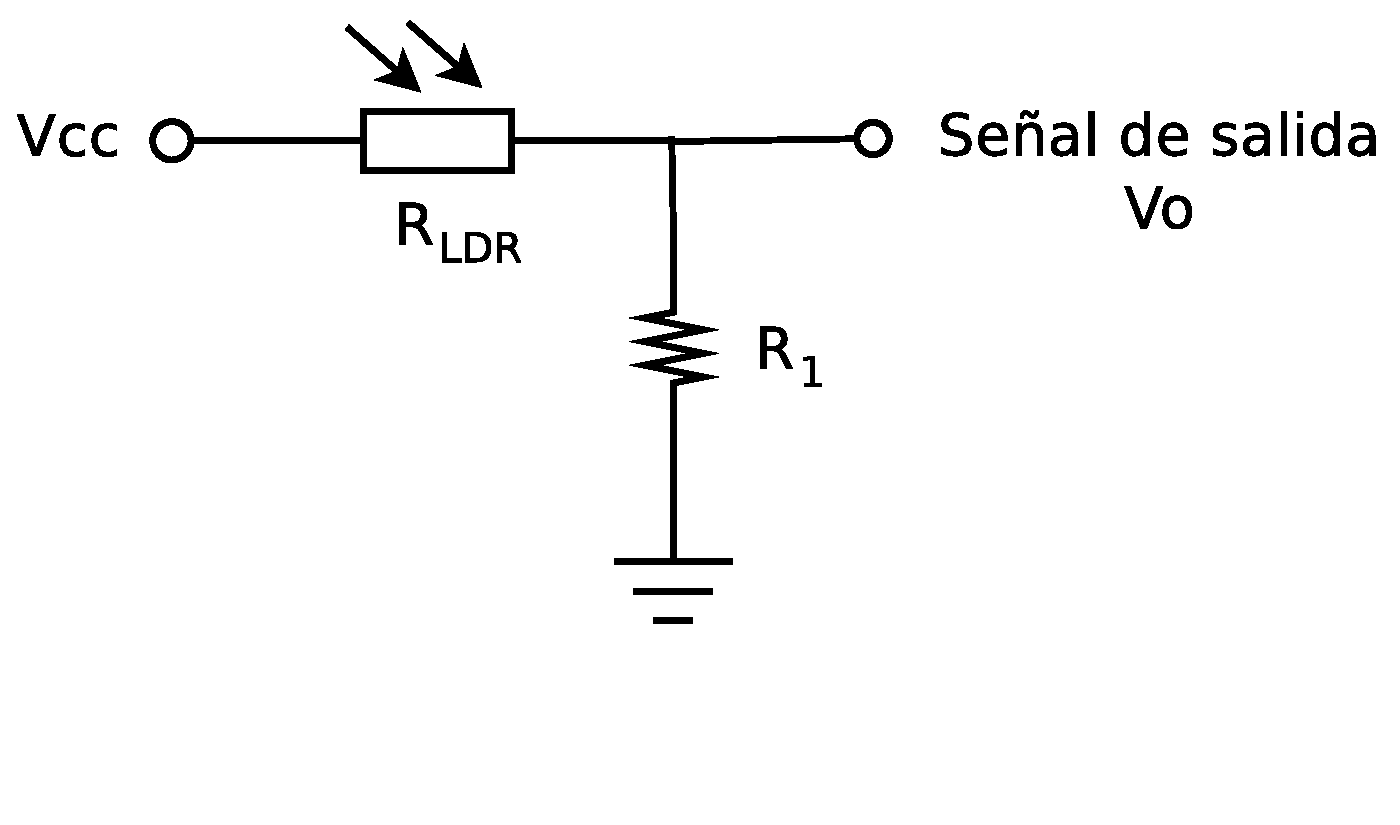
\includegraphics[width=\textwidth]{Figures/LDR.eps}
    \caption{Divisor de voltaje.}
    \label{fig:LDR}
  \end{subfigure}
  \qquad\qquad
  \begin{subfigure}[b]{0.43\textwidth}
    \centering
    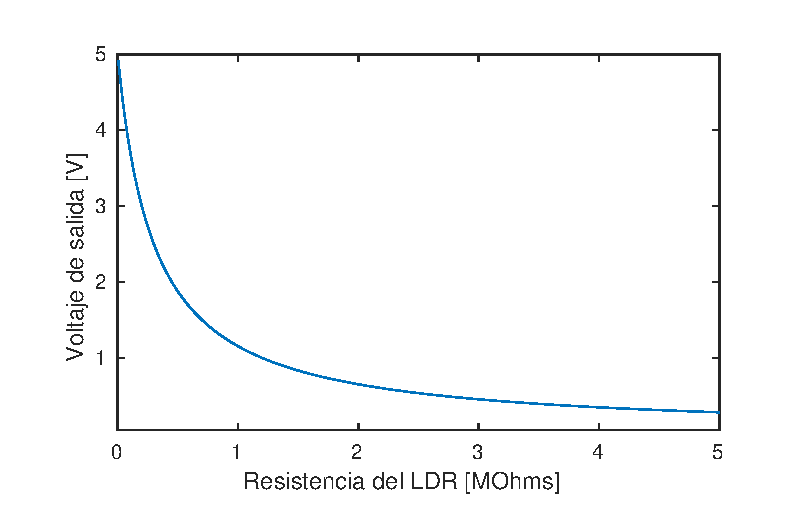
\includegraphics[width=\textwidth]{Figures/LDR_Vo.eps}
    \caption{Voltaje de salida.}
    \label{fig:LDRVo}
  \end{subfigure}
\caption{Sensores de luz basados en LDR.}
\end{figure}

La idea de estos sensores es medir diferencias de luz a cada lado del robot de modo que puedan implementarse fototaxias (ver práctica 10), por lo que uno de los sensores debe colocarse al lado izquierdo del robot y el otro, al lado derecho. 

\subsection{Sensor de batería}
Construya un divisor de voltaje cuya salida sea la mitad del voltaje de entrada. En el circuito de la figura \ref{fig:VoltDiv} el voltaje de salida $V_o$ está dado por
\[V_o = \ddfrac{R2}{R1 + R2}V_i\]
por lo que, si las resistencias R1 y R2 son iguales, el voltaje de salida $V_o$ será la mitad del voltaje de entrada $V_i$ (que en este caso será el voltaje de la batería). Teóricamente, R1 y R2 podrían tomar cualquier valor siempre y cuando sean iguales, sin embargo, dado que dicha señal será conectada a un convertidor ADC del Arduino Uno, es necesario tomar en cuenta la impedancia de entrada de dicho convertidor. 

Considere el circuito de la figura \ref{fig:VoltDivADC}. La señal de salida $V_o$ está dada por
\[V_o = \ddfrac{\left(R2^{-1} + R_{ADC}^{-1}\right)^{-1}}{R1 + \left(R2^{-1} + R_{ADC}^{-1}\right)^{-1}}V_i\]
Dado que la resistencia R2 está conectada en paralelo con la impedancia de entrada $\textrm{R}_{ADC}$ del convertidor analógico-digital, entre más pequeñas sean R1 y R2, menor será la alteración provocada por $\textrm{R}_{ADC}$, sin embargo, entre más pequeñas sean R1 y R2, mayor será el consumo de corriente. Por lo tanto, R1 y R2 se deben seleccionar equilibrando exactitud y consumo de corriente. 

\begin{figure}
  \centering
  \begin{subfigure}[b]{0.43\textwidth}
    \centering
    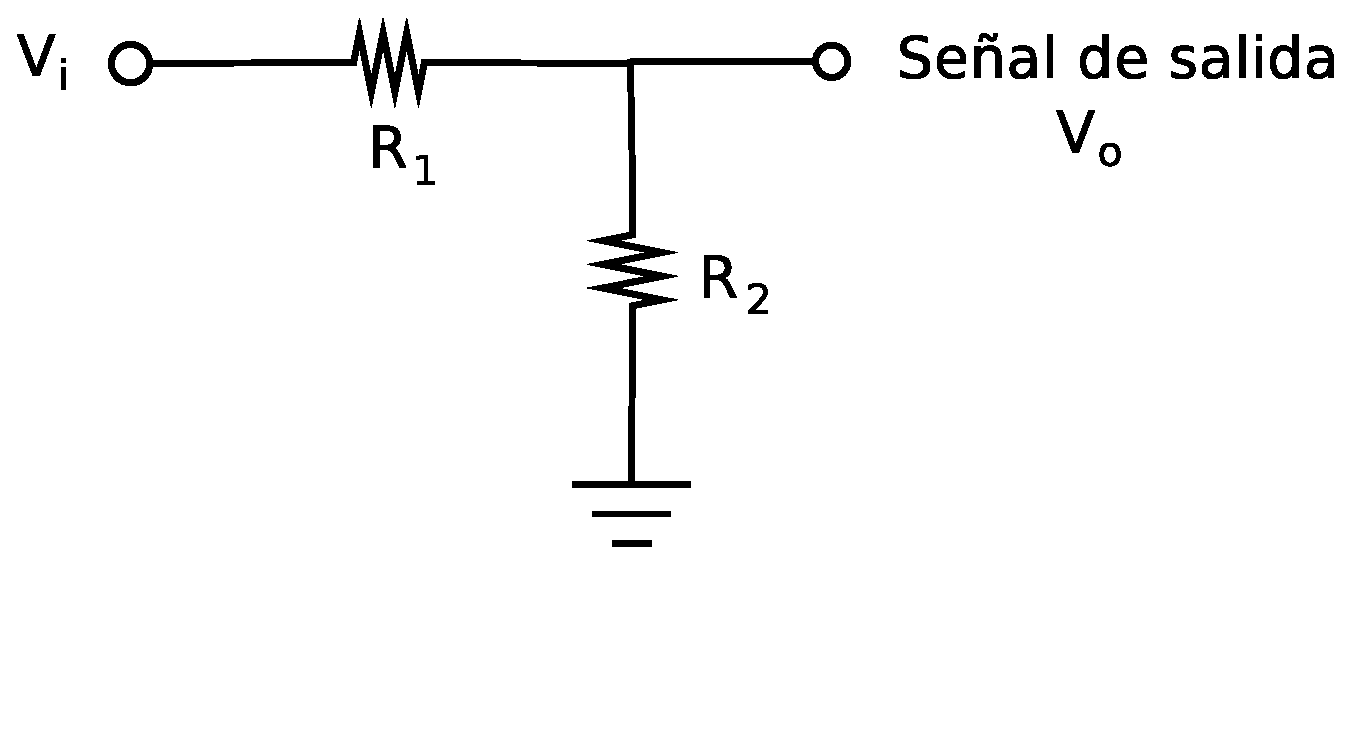
\includegraphics[width=\textwidth]{Figures/VoltDiv.eps}
    \caption{Divisor de voltaje para reducir a la mitad el voltaje de entrada.}
    \label{fig:VoltDiv}
  \end{subfigure}
  \qquad\qquad
  \begin{subfigure}[b]{0.43\textwidth}
    \centering
    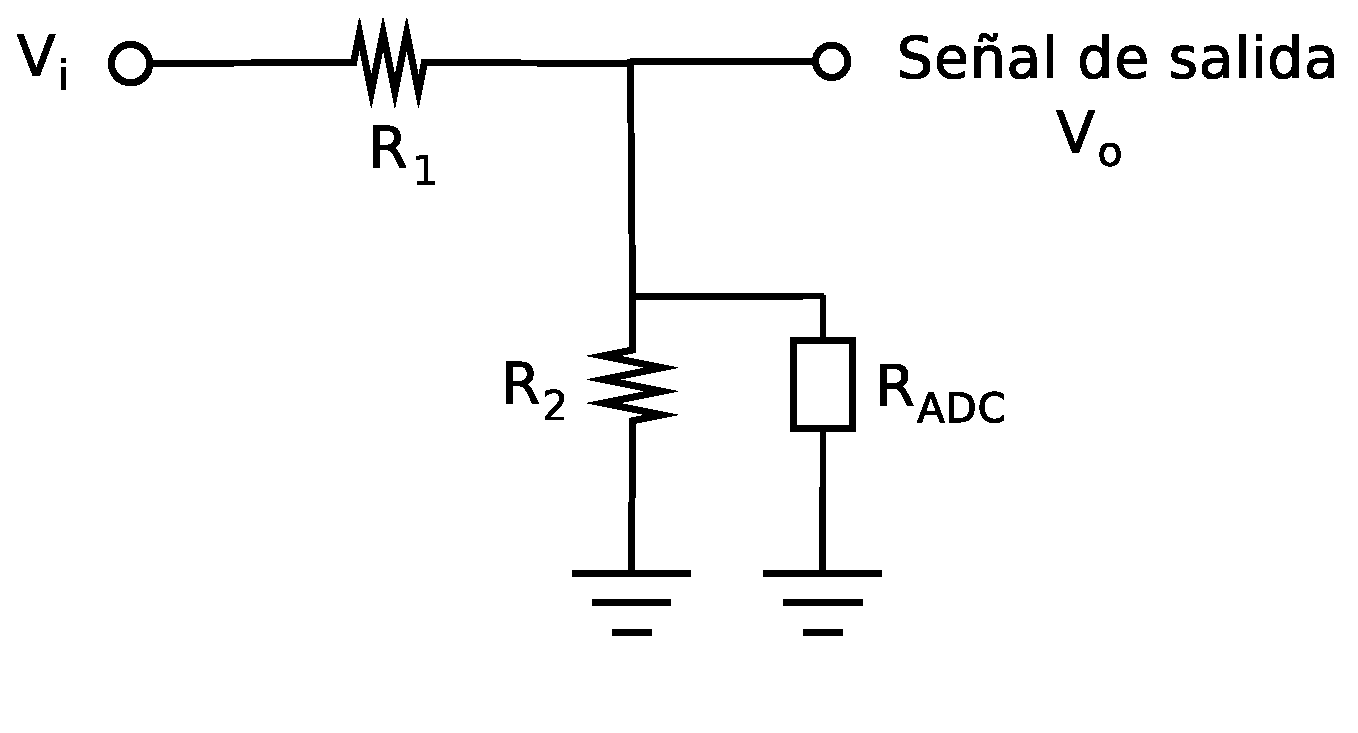
\includegraphics[width=\textwidth]{Figures/VoltDivADC.eps}
    \caption{Divisor considerando la impedancia del convertidor analógico-digital.}
    \label{fig:VoltDivADC}
  \end{subfigure}
\caption{Circuito para sensar batería.}
\end{figure}

\subsection{Conexión de los sensores al Arduino Uno}
Conecte la salida de los sensores de luz izquierdo y derecho a los pines analógicos de entrada A0 y A1 del Arduino Uno.  Conecte la salida del sensor de batería al pin A2. Alimente con 5V el circuito TMP36 y conecte su salida al pin A3. La razón para usar estos pines es que los demás, digitales y analógicos, serán usados para otros dispositivos, como se muestra en la tabla \ref{tab:PinUsage}.

\begin{table}
\centering
\begin{tabular}{rll}
\hline
Pin & Dispositivo conectado & Descripción\\
\hline
0 & Serial Rx  & Comunicación serial con la RaspberryPi\\
1 & Serial Tx  & Comunicación serial con la RaspberryPi\\
2 & Sensor SD0 & Sensor de distancia binario\\
3 & Motor MA1  & Señal PWM para control del motor izquierdo\\
4 & Sensor SD1 & Sensor de distancia binario\\
5 & Motor MA2  & Señal PWM para control del motor izquierdo\\
6 & Motor MB1  & Señal PWM para control del motor derecho\\
7 & Sensor SD2 & Sensor de distancia binario\\
8 & Sensor SD3 & Sensor de distancia binario\\
9 & Motor MB2  & Señal PWM para control del motor derecho\\
10& Sensor SD4 & Sensor de distancia binario\\
11& Sensor SD5 & Sensor de distancia binario\\
12& Sensor SD6 & Sensor de distancia binario\\
13& Sensor SD7 & Sensor de distancia binario\\
A0& Sensor SLL & Sensor de luz izquierdo\\
A1& Sensor SLR & Sensor de luz derecho\\
A2& Sensor SB  & Sensor de batería\\
A3& Sensor ST  & Sensor de temperatura\\
A4& I2C SCL    & Comunicación con el acelerómetro\\
A5& I2C SDA    & Comunicación con el acelerómetro\\
\hline
\end{tabular}
\caption{Uso de los pines de la tarjeta Arduino Uno}
\label{tab:PinUsage}
\end{table}

\subsection{Nodo que publica los valores de los sensores}
Implemente un nodo en la tarjeta Arduino Uno (siguiendo un procedimiento similar a la práctica 3) que publique un tópico de tipo \texttt{std\_msgs::Float32MultiArray} con el nombre \texttt{/minirobot/hardware/sensors} que contenga las lecturas de los sensores de luz, batería y temperatura, además de los sensores de distancia construidos en la práctica 4. El tamaño del arreglo de flotantes contenido en el mensaje \textbf{debe ser 15}. Recuerde que el tamaño del arreglo se especifica en la variable \texttt{data\_length} del mensaje a enviar. Es importante que \textbf{el tamaño del arreglo sea 15} para el correcto funcionamiento de la GUI donde se desplegarán los valores de los sensores. 

El arreglo de flotantes del mensaje a publicar debe contener las lecturas de los sensores en el siguiente orden (ver tabla \ref{tab:PinUsage} para los nombres de los sensores):
\begin{verbatim}
  {SD0  SD1  SD2  SD3  SD4  SD5  SD6  SD7   0  0  0   SLL  SLR  ST  SB}
\end{verbatim}

De los quince datos, los primeros ocho corresponden a los sensores de distancia, los siguietes tres datos deben ser cero (se utilizarán en la siguiente práctica para la lectura del acelerómetro) y los últimos cuatro deben contener las lecturas de los sensores de luz izquierdo y derecho, sensor de temperatura y sensor de batería, en ese orden. Por ejemplo, suponga que los sensores SD0, SD2 y SD3 detectan objetos cercanos, los voltajes de los sensores de luz son 3.5V y 4.5V, la batería tiene un nivel de 8.0V y el sensor de temperatura entrega una salida de 0.8V. Dado que el Arduino Uno tiene un ADC de 10 bits alimentado a 5V, el contenido del arreglo debería ser (recuerde que la batería pasa por un divisor de voltaje):
\begin{verbatim}
  {0  1  0  0  1  1  1  1  0  0  0  717  922  164  819}
\end{verbatim}

con lo que la GUI desplegará algo como lo que se muestra en la figura \ref{fig:Example}. Para correr la GUI y visualizar los datos, en una nueva terminal, ejecute el comando

\begin{lstlisting}[language=bash]
$  rosrun mini_robot_gui mini_robot_gui_node
\end{lstlisting}

\begin{figure}
  \centering
  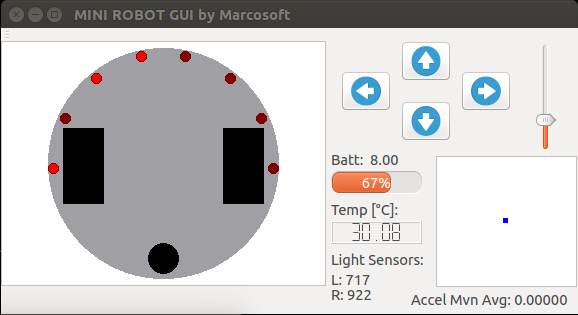
\includegraphics[width=0.7\textwidth]{Figures/SensorExample.png}
  \caption{Ejemplo de lectura de sensores. SD0, SD2 y SD3 detectan objetos cercanos. Sensores de luz con salidas de 3.5V y 4.5V, sensor de temperatura entrega 0.8V y batería con 8.0V.}
  \label{fig:Example}
\end{figure}

\section{Evaluación}
\begin{itemize}
\item Los cuatro sensores (dos de luz, batería y temperatura), junto con los ocho de distancia de la práctica 4, deben funcionar correctamente.
\item Todos los sensores deben estar montados en el robot.
\item El correcto funcionamiento de todos los sensores se verificará con la GUI.
\item Los sensores de luz deben mostrar variaciones de cuando menos 2V ante dos condiciones: tapados con las manos (condición de obscuridad) y descubiertos (condición luminosa).
\item El sensor de batería debe tener valores ``razonables'', es decir, puesto que se usará una batería LiPo de dos celdas, el voltaje leído no debería ser menor a 7.0V ni mayor a 8.4V.
\item El sensor de temperatura también debe mostrar valores ``razonables''. La GUI ya hace la transformación a \si{\degree}C con base en las especificaciones del TMP36, por lo que se esperan lecturas cercanas a la temperatura ambiente. 
\end{itemize}

\end{document}

%%% Local Variables:
%%% mode: latex
%%% TeX-master: t
%%% End:
